% AuxForge - Slide deck (Beamer)
% Dựng theo docs/SLIDE_AND_REPORT_GUIDE.md §3 (outline 14 slide).
% Nguồn số liệu: README.md, docs/PIPELINE.md, docs/PHYSICS_AND_ML.md, docs/LIMITATIONS.md (tính đến 2026-08-05).
% Biên dịch: tectonic docs/slides/auxforge_slides.tex   (hoặc xelatex)

\documentclass[aspectratio=169,11pt]{beamer}

% ---- Fonts (XeTeX/tectonic, giống outputs/phase5/reports/bao_cao_so_lieu_fix1_fix2.tex) ----
\usepackage{fontspec}
\setmainfont{Noto Sans}
\newfontfamily\notomono{Noto Sans Mono}

\usepackage{amsmath,amssymb}
\usepackage{graphicx}
\usepackage{booktabs}
\usepackage{tikz}
\usetikzlibrary{arrows.meta,positioning,shapes.geometric}

\usetheme{Madrid}
\usecolortheme{whale}
\usefonttheme{professionalfonts}
\setbeamertemplate{navigation symbols}{}
\setbeamertemplate{caption}[numbered]

% ---- Palette ----
\definecolor{okGreen}{HTML}{1e7d34}
\definecolor{warnAmber}{HTML}{b8860b}
\definecolor{noRed}{HTML}{a4262c}
\definecolor{boxBlue}{HTML}{2a5599}

\setbeamercolor{block title example}{bg=okGreen!85!black,fg=white}
\setbeamercolor{block body example}{bg=okGreen!10,fg=black}
\setbeamercolor{block title alerted}{bg=warnAmber!85!black,fg=white}
\setbeamercolor{block body alerted}{bg=warnAmber!12,fg=black}
\setbeamercolor{block title}{bg=noRed!80!black,fg=white}
\setbeamercolor{block body}{bg=noRed!8,fg=black}

\title[AuxForge]{AuxForge}
\subtitle{Tối ưu hóa Topology cho Thiết kế ngược Vi cấu trúc Vật liệu Auxetic}
% TODO: điền tên tác giả/nhóm thật trước khi trình bày.
\author{AuxForge Team}
\institute{Phiên bản \texttt{v1.4.0} - nhánh \texttt{main}}
\date{Cập nhật tính đến 2026-08-05}

\begin{document}

% =====================================================================
\begin{frame}
  \titlepage
\end{frame}

% ===================== 2. Motivation & Bài toán =======================
\begin{frame}{Vật liệu Auxetic \& Bài toán Thiết kế ngược}
  \begin{itemize}
    \item \textbf{Vật liệu auxetic}: hệ số Poisson âm ($\nu<0$) - kéo dãn theo một phương thì \textbf{NỞ RA} theo phương vuông góc, ngược với vật liệu thông thường ($\nu>0$).
    \item Hành vi này đến từ \textbf{hình học vi cấu trúc} của ô đơn vị tuần hoàn (unit cell), không phải từ thành phần hóa học của vật liệu nền.
    \item \textbf{Bài toán trung tâm}: cho một vật liệu nền đẳng hướng thông thường ($\nu_0>0$), tìm cách phân bố vật liệu/lỗ rỗng trong một ô đơn vị 2D sao cho vật liệu đồng nhất hóa có $\nu_{12}, \nu_{21}$ càng âm càng tốt.
    \item Giải bằng \textbf{SIMP} (Solid Isotropic Material with Penalization) - tối ưu hóa topology kinh điển (Sigmund 2001; Andreassen et al. 2011).
    \item \textbf{Mục tiêu dự án}: \textbf{thiết kế ngược (inverse design)} - cho trước $(\nu_{12},\nu_{21})$ mục tiêu, sinh ra hình học đạt được nó, bằng mô hình sinh có điều kiện (cVAE) huấn luyện trên dữ liệu do chính engine SIMP tạo ra.
  \end{itemize}
\end{frame}

% ===================== 3. Kiến trúc tổng thể (sơ đồ 2.1) ================
\begin{frame}{Kiến trúc Pipeline 8-Phase}
  \centering
  \resizebox{\textwidth}{!}{%
  \begin{tikzpicture}[
      node distance=6mm and 6mm,
      box/.style={rectangle, rounded corners, draw, thick, align=center,
                  font=\scriptsize, minimum height=1.5cm, text width=2.6cm},
      >=Latex
    ]
    \node[box, fill=boxBlue!12] (p0) {Phase 0\\SIMP Engine\\\textcolor{okGreen}{$\checkmark$ Ổn định}};
    \node[box, fill=boxBlue!12, right=of p0] (p1) {Phase 1\\LHS Screening\\\textcolor{okGreen}{$\checkmark$ volfrac chi phối}};
    \node[box, fill=boxBlue!12, right=of p1] (p2) {Phase 2\\Multi-Batch DOE\\\textcolor{okGreen}{$\checkmark$ 7.920 mẫu, 91,9\% aux.}};
    \node[box, fill=boxBlue!12, right=of p2] (p3) {Phase 3\\Dataset Build\\\textcolor{okGreen}{$\checkmark$ 57.216/2.044/2.044}};
    \node[box, fill=okGreen!15, right=of p3] (p4) {Phase 4\\CNN Surrogate\\\textcolor{okGreen}{$\checkmark$ R\textsuperscript{2} 0,93--0,98}};

    \node[box, fill=okGreen!25, below=of p4] (p5) {Phase 5\\Conditional VAE\\\textcolor{okGreen}{$\checkmark\checkmark$ R\textsuperscript{2}=0,995--0,999}};
    \node[box, fill=boxBlue!12, left=of p5] (p6) {Phase 6\\Hậu xử lý \& FE verify\\\textcolor{okGreen}{$\checkmark$}};
    \node[box, fill=boxBlue!12, left=of p6] (p7) {Phase 7\\Active Learning\\\textcolor{okGreen}{$\checkmark$ Không cải thiện}};
    \node[box, fill=warnAmber!18, left=of p7] (p8) {Phase 8\\Xác thực \& Đóng gói\\\textcolor{warnAmber}{Một phần}};

    \draw[->] (p0) -- (p1);
    \draw[->] (p1) -- (p2);
    \draw[->] (p2) -- (p3);
    \draw[->] (p3) -- (p4);
    \draw[->] (p4) -- (p5);
    \draw[->] (p5) -- (p6);
    \draw[->] (p6) -- (p7);
    \draw[->] (p7) -- (p8);
  \end{tikzpicture}}
  \vspace{2mm}
  \small Phase 1--4: hoàn thành, xác thực trên dữ liệu thực. Phase 5: sửa tận gốc bằng differentiable real-physics. Chi tiết từng phase con: \texttt{html/dashboards/workflow.html}.
\end{frame}

% ===================== 4. SIMP cơ bản & 11 seed (sơ đồ 2.2) ============
\begin{frame}{SIMP Engine \& 11 Hình học Seed}
  \begin{columns}[T]
    \begin{column}{0.46\textwidth}
      \centering
      \resizebox{!}{4.5cm}{%
      \begin{tikzpicture}[
          node distance=3mm,
          box/.style={rectangle, rounded corners, draw, align=center,
                      font=\tiny, minimum height=0.8cm, text width=2.6cm},
          >=Latex
        ]
        \node[box] (a) {Seed\\Generation};
        \node[box, below=of a] (b) {FE Analysis};
        \node[box, below=of b] (c) {Homogenization\\$U_{tot}=U_0+\chi$};
        \node[box, below=of c] (d) {Objective \&\\Sensitivity};
        \node[box, below=of d] (e) {Density/Sens.\\Filtering};
        \node[box, below=of e] (f) {OC Update};
        \node[diamond, draw, below=of f, font=\tiny, text width=2.1cm, align=center, aspect=2] (g) {Hội tụ?};
        \node[box, below=of g] (h) {Kết thúc: $x_{phys}, Q,$\\$\nu_{12}/\nu_{21}$};
        \draw[->] (a)--(b); \draw[->] (b)--(c); \draw[->] (c)--(d);
        \draw[->] (d)--(e); \draw[->] (e)--(f); \draw[->] (f)--(g);
        \draw[->] (g)--(h) node[midway, right, font=\tiny] {Rồi};
        \draw[->] (g.west) -- ++(-1.0,0) |- (b.west) node[midway, above, font=\tiny] {Chưa};
      \end{tikzpicture}}
      \vspace{1mm}
      {\scriptsize $c = Q_{12} - \mu(Q_{11}+Q_{22}) + \text{penalty}$\\
       penalty khi $Q_{11}$ hoặc $Q_{22} < \delta = 0{,}1\!\cdot\!\text{volfrac}\!\cdot\!E_0$}
    \end{column}
    \begin{column}{0.52\textwidth}
      \scriptsize
      \textbf{Tỷ lệ thành công auxetic* theo seed} (n=7.920, Phase 2 DOE):
      \begin{tabular}{@{}lr@{}}
        \toprule
        Seed & \% auxetic \\ \midrule
        \texttt{grid\_circular\_voids} & 99,4\% \\
        \texttt{nine\_circle} & 98,9\% \\
        \texttt{square} & 94,0\% \\
        \texttt{circle} & 93,8\% \\
        \texttt{small\_square\_cross} & 93,1\% \\
        \texttt{cross\_rectangular} & 93,3\% \\
        \texttt{four\_circle} & 87,9\% \\
        \texttt{hourglass} & 67,8\% \\
        \texttt{hexagonal} & 64,4\% \\
        \texttt{circle\_half\_quarter} & 61,7\% \\
        \texttt{reentrant\_bowtie} & 48,6\% \\
        \bottomrule
      \end{tabular}
      \vspace{1mm}\\
      *$\nu_{12}<0$ \textbf{và} $\nu_{21}<0$. \texttt{reentrant\_bowtie}/\texttt{hexagonal}: khó đẩy auxetic nhất.
    \end{column}
  \end{columns}
\end{frame}

% ===================== 5. Phase 1 - Screening ==========================
\begin{frame}{Phase 1 - LHS Screening: \texttt{volfrac} chi phối}
  \begin{columns}[T]
    \begin{column}{0.5\textwidth}
      \centering
      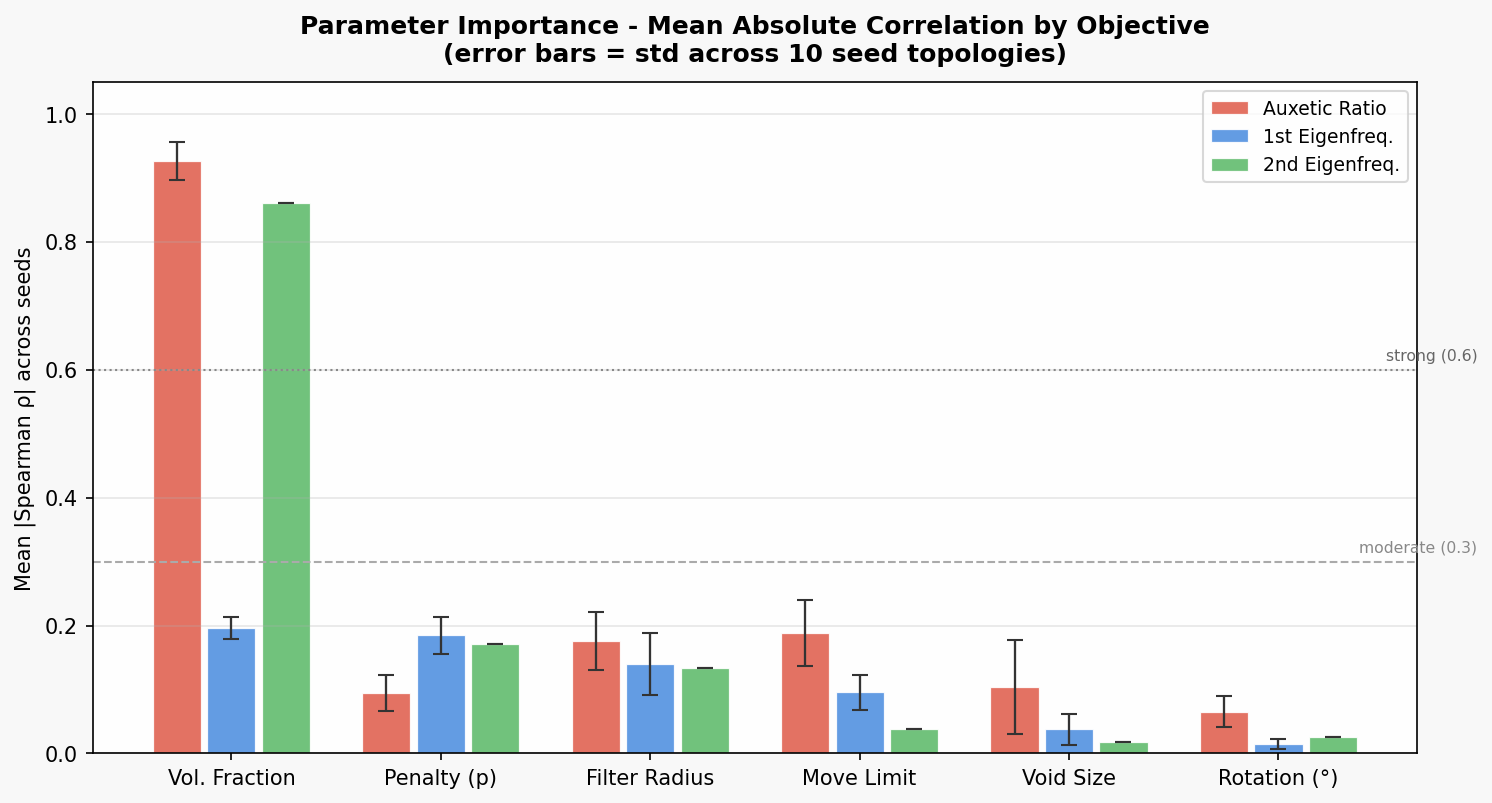
\includegraphics[width=\textwidth]{../../outputs/figures/design_correlations/barplot_importance.png}
    \end{column}
    \begin{column}{0.5\textwidth}
      \centering
      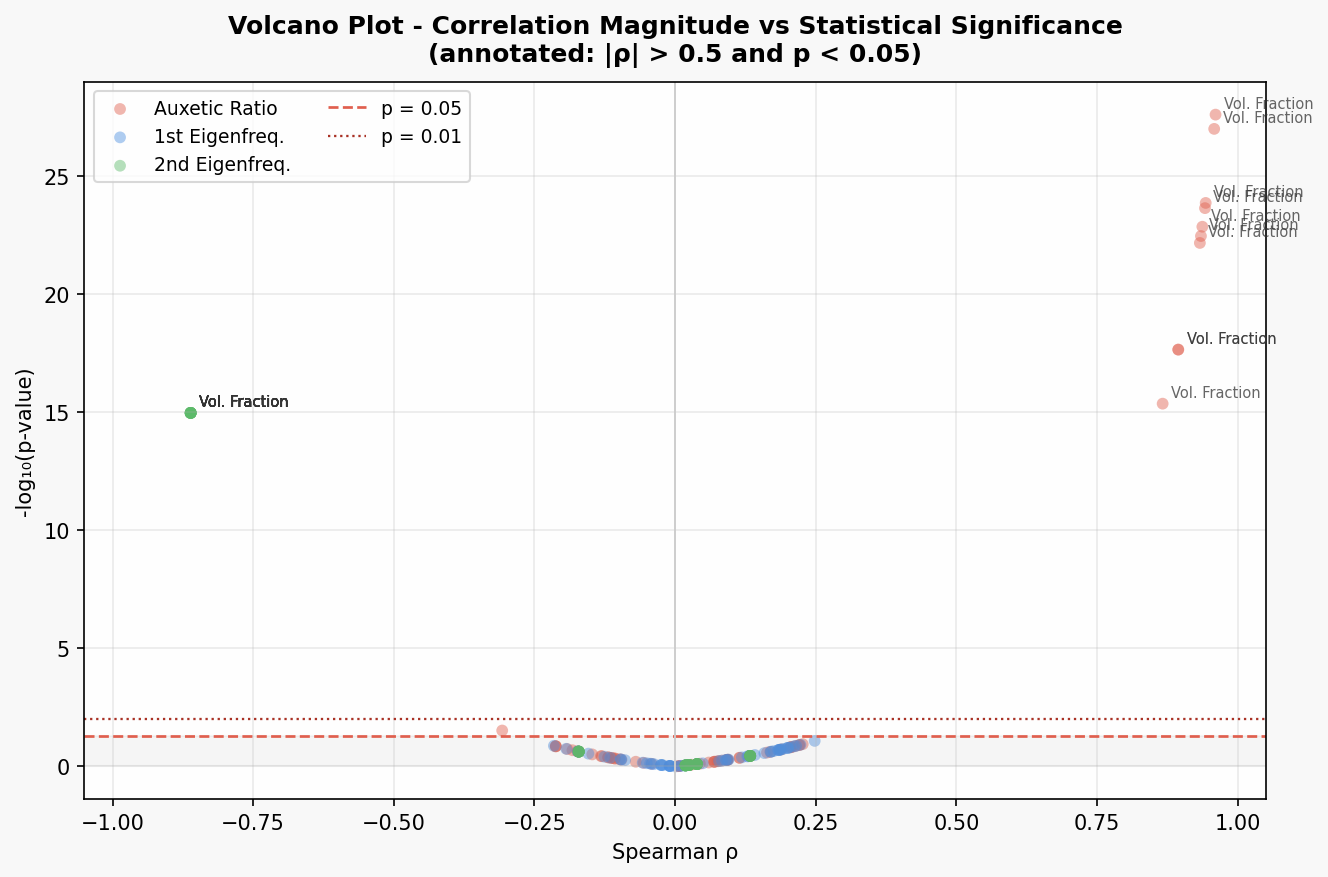
\includegraphics[width=\textwidth]{../../outputs/figures/design_correlations/volcano_plot.png}
    \end{column}
  \end{columns}
  \vspace{2mm}
  \begin{itemize}\small
    \item Quét Latin Hypercube Sampling trên \texttt{volfrac, penal, rmin, move, void\_size\_frac, rotation\_deg}.
    \item Tương quan Spearman: \textbf{\texttt{volfrac} là tham số chi phối} ($r\approx 0{,}87$--$0{,}96$).
    \item \texttt{move}, \texttt{rmin}, \texttt{void\_size\_frac}: không có ý nghĩa thống kê.
  \end{itemize}
\end{frame}

% ===================== 6. Phase 2 - Adaptive DOE ========================
\begin{frame}{Phase 2 - Multi-Batch Adaptive DOE}
  \centering\scriptsize
  \begin{tabular}{@{}clrrr@{}}
    \toprule
    Lô & Chiến lược & Số mẫu & \% Auxetic & $\nu_{12}$ tốt nhất \\ \midrule
    1 & Sobol (khám phá) & 1.320 & 74,9\% & $-0{,}612$ \\
    2 & Sobol (khám phá) & 600 & 79,7\% & $-0{,}519$ \\
    3 & Sobol (khám phá) & 720 & 71,8\% & $-0{,}565$ \\
    4 & Optimized LHS (tinh chỉnh) & 1.056 & 83,6\% & $-0{,}605$ \\
    5 & Optimized LHS (tinh chỉnh) & 1.067 & 85,7\% & $-0{,}752$ \\
    6 & Optimized LHS (tinh chỉnh) & 1.045 & 85,4\% & $-0{,}649$ \\
    7 & Optimized LHS (tinh chỉnh) & 1.056 & 85,3\% & $-0{,}621$ \\
    8 & Optimized LHS (tinh chỉnh) & 1.056 & 87,8\% & $\mathbf{-0{,}807}$ \\
    \bottomrule
  \end{tabular}
  \vspace{2mm}
  \begin{itemize}\small
    \item \textbf{8/8 lô + batch 11 rebuild}, tổng 7.920 mẫu, \textbf{tỷ lệ hội tụ FE 100\%}.
    \item 2026-07-24: manufacturability hầu như không tương quan với tham số DOE liên tục ($|r|<0{,}12$) - biến chi phối là \textbf{SEED} (7,9\%--62,8\%).
    \item Sửa lỗi hoán vị \texttt{dQ} + rebuild 2.160 mẫu $\Rightarrow$ auxetic rate toàn dataset \textbf{82,1\%$\to$91,9\%}.
  \end{itemize}
\end{frame}

% ===================== 7. Phase 3 - Dataset =============================
\begin{frame}{Phase 3 - Xây dựng Dataset}
  \begin{itemize}
    \item \textbf{QC}: loại bỏ 2.662/7.920 mẫu (\textbf{33,6\%}) - nhãn dao động/rời rạc/ngoài khoảng vật lý hợp lệ.
    \item \textbf{Chia train/val/test 70/15/15}, phân tầng theo seed (chống rò rỉ dữ liệu giữa các tập).
    \item \textbf{Tăng cường đối xứng} (chỉ áp dụng cho train): xoay $90^\circ/270^\circ$ hoán đổi $\nu_{12}\leftrightarrow\nu_{21}$; xoay $180^\circ$/lật giữ nguyên nhãn.
    \item \textbf{Rebuild v2 (2026-07-25)}: sinh thêm mẫu độc lập + gộp với pool sạch cũ.
    \item \textbf{Dataset production hiện hành}: train = \textbf{57.216} / val = \textbf{2.044} / test = \textbf{2.044} mẫu.
  \end{itemize}
\end{frame}

% ===================== 8. Phase 4 - CNN Surrogate =======================
\begin{frame}{Phase 4 - CNN Surrogate}
  \begin{itemize}
    \item Kiến trúc: $4\times$ khối \texttt{Conv(3x3)+BatchNorm+ReLU+MaxPool} $\to$ global average pool $\to$ nối one-hot seed $\to$ 2 lớp FC $\to$ 3 đầu ra ($\nu_{12}, \nu_{21}$, volfrac\_achieved).
    \item Vai trò: hàm mất mát khả vi, rẻ (\texttt{property\_consistency\_loss}) để huấn luyện Phase 5 - \textbf{không} thay thế FE trong đánh giá cuối cùng.
  \end{itemize}
  \vspace{2mm}
  \centering
  \texttt{surrogate\_v2.pt} - R\textsuperscript{2} trên test set v2 (n=2.044):
  \begin{tabular}{@{}lc@{}}
    \toprule
    Target & R\textsuperscript{2} \\ \midrule
    $\nu_{12}$ & \textbf{0,974} \\
    $\nu_{21}$ & \textbf{0,964} \\
    volfrac\_achieved & \textbf{0,983} \\
    \bottomrule
  \end{tabular}
  \vspace{2mm}\\
  \small CI tính bằng bootstrap percentile (\texttt{bootstrap\_ci.py}); ở phiên bản trước (\texttt{surrogate\_best.pt}, n=1.184) CI đo được rất hẹp - cỡ mẫu lớn nên R\textsuperscript{2} đáng tin, không phải điểm ước lượng may rủi.
\end{frame}

% ===================== 9. Phase 5 - cVAE & Surrogate Exploitation =======
\begin{frame}{Phase 5 - cVAE \& ``Surrogate Exploitation''}
  \begin{columns}[T]
    \begin{column}{0.34\textwidth}
      \scriptsize
      \textbf{cVAE}: Encoder (4 khối Conv) $\to (\mu,\log\sigma^2)$; Decoder \texttt{ConvTranspose2d} đối xứng.
      \[
        \mathcal{L} = \text{BCE} + \beta\cdot\text{KL} + \gamma\cdot\mathcal{L}_{prop}
      \]
      \vspace{1mm}
      \textit{Câu chuyện khoa học chính của dự án - xem sơ đồ bên phải.}
    \end{column}
    \begin{column}{0.66\textwidth}
      \centering
      \resizebox{\textwidth}{!}{%
      \begin{tikzpicture}[
          node distance=2mm,
          box/.style={rectangle, rounded corners, draw, align=center,
                      font=\tiny, minimum height=0.9cm, text width=8.6cm},
          >=Latex
        ]
        \node[box, fill=noRed!12] (a) {Surrogate-only R\textsuperscript{2} cao (qua CNN đóng băng)};
        \node[box, fill=noRed!20, below=of a] (b) {FE thật kiểm tra lại $\to$ R\textsuperscript{2} \textbf{ÂM SÂU}};
        \node[box, fill=warnAmber!18, below=of b] (c) {Chẩn đoán: decoder học đánh lừa CNN, không sinh hình học đúng vật lý};
        \node[box, fill=warnAmber!12, below=of c] (d) {Thử self-play, ensemble surrogate $\to$ \textbf{KHÔNG đủ}};
        \node[box, fill=boxBlue!15, below=of d] (e) {Giải pháp tận gốc: differentiable real-physics (FE-solve + gradient trong loop)};
        \node[box, fill=okGreen!22, below=of e] (f) {\texttt{cvae\_realphysics.pt}: R\textsuperscript{2}(FE,n=789)=\textbf{0,999}, hit-rate=\textbf{98,7\%}};
        \draw[->] (a)--(b); \draw[->] (b)--(c); \draw[->] (c)--(d);
        \draw[->] (d)--(e); \draw[->] (e)--(f);
      \end{tikzpicture}}
    \end{column}
  \end{columns}
\end{frame}

% ===================== 10. Phase 5 - Kết quả & mở rộng ==================
\begin{frame}{Phase 5 - Kết quả \& Mở rộng}
  \centering\scriptsize
  So sánh checkpoint, đo trên \textbf{cùng test set v2 (n=300)}:
  \begin{tabular}{@{}lccc@{}}
    \toprule
    Checkpoint & R\textsuperscript{2}(FE) oracle & Hit rate single-shot & Frac. manufacturable \\ \midrule
    \texttt{cvae\_v2\_finetuned.pt} (train v2) & 0,9953 & \textbf{0,997} & 0,247 \\
    \texttt{cvae\_realphysics.pt} (train cũ) & \textbf{0,9984} & 0,983 & \textbf{0,280} \\
    \bottomrule
  \end{tabular}
  \vspace{2mm}\\
  \raggedright\small
  \begin{itemize}
    \item \textbf{Khuyến nghị production: \texttt{cvae\_v2\_finetuned.pt}} (nhất quán với dataset v2, 57.216 mẫu). \texttt{cvae\_realphysics.pt} giữ làm tham chiếu lịch sử.
    \item \textbf{Mở rộng (merge \texttt{main} 2026-07-25):} \texttt{volfrac}/\texttt{void\_size\_frac} làm condition \emph{optional} - \texttt{condition\_dim} $2\to 6$, qua presence-mask + condition-dropout (\texttt{--extended-condition}).
    \item \textbf{Chấm điểm tổng hợp} trong \texttt{best\_of\_n\_eval.py}: \texttt{composite\_score} = $0{,}6\!\cdot\!\text{accuracy} + 0{,}3\!\cdot\!\text{manuf} + 0{,}1\!\cdot\!\text{aesthetic}$ thay cho $\arg\min|\Delta\nu_{12}|$ thuần túy.
  \end{itemize}
\end{frame}

% ===================== 11. Phase 6-8 =====================================
\begin{frame}{Phase 6--8 - Hậu xử lý \& Xác thực}
  \begin{itemize}
    \item \textbf{Phase 6}: nhị phân hoá + \texttt{force\_periodic()} + lọc manufacturability (connectivity/min-feature/periodicity) + lọc bằng FE thật (\texttt{best\_of\_n\_eval.py}).
    \item \textbf{Phase 7 (kết luận 2026-07-31)}: active-learning loop chạy production - \textbf{không cải thiện} checkpoint đã gần trần (mean\_abs\_error 0,0246$\to$0,0686 sau 1 vòng); giữ nguyên checkpoint production.
    \item \textbf{Phase 8.1 - đối chiếu FE độc lập}: \texttt{scikit-fem} khớp engine nội bộ tới $1\text{e-}9$ - \textbf{R\textsuperscript{2}=1,000000 (n=24)} - xác nhận đúng vật lý, không chỉ nhất quán nội bộ.
    \item \textbf{Phase 8.3 - thư viện thiết kế}: 24 thiết kế, \textbf{hit-rate 100\%}, \textbf{87,5\%} xác nhận manufacturable.
    \item \textbf{8.2 (biến dạng lớn), 8.5 (chuẩn bị STL)}: chưa làm (tùy chọn, xem slide Giới hạn).
  \end{itemize}
\end{frame}

% ===================== 12. Phạm vi claim khoa học (bắt buộc) ============
\begin{frame}{Phạm vi Claim Khoa học}
  \small
  \begin{block}{\textcolor{white}{$\checkmark$ Được ủng hộ bởi bằng chứng}}
    Engine FE/homogenization đúng vật lý (đối chiếu \texttt{scikit-fem}, R\textsuperscript{2}=1,000000, n=24) $\bullet$ checkpoint hiện tại dự đoán đúng \textbf{DẤU} $(\nu_{12},\nu_{21})$ ở tỉ lệ cao (n=789) $\bullet$ cVAE sinh thiết kế \textbf{không} sao chép training set (novelty) $\bullet$ cVAE vượt trội retrieval trên trục đổi dấu \textbf{ngoài phân phối train} (R\textsuperscript{2}=0,42 vs 0,06, n=12).
  \end{block}
  \begin{alertblock}{\textcolor{white}{$\sim$ Chưa được ủng hộ (dù có thể đúng)}}
    Proxy $Q_{12}$ tương đương mục tiêu auxetic ``thật'' dưới mọi điều kiện xoay $\bullet$ cVAE vượt trội retrieval về độ chính xác \textbf{trong-phân-phối} (retrieval còn thắng) $\bullet$ cVAE ngoại suy được cường độ auxetic vượt xa phạm vi train $\bullet$ \texttt{hit\_rate} như chỉ số độc lập (base rate $\approx$92\% auxetic).
  \end{alertblock}
  \begin{block}{\textcolor{white}{$\times$ Không claim}}
    ``Đã giải quyết inverse design'' $\bullet$ ``cVAE tốt hơn phương pháp classical trong mọi trường hợp'' $\bullet$ ``surrogate có thể thay FE ở vùng chưa kiểm chứng''.
  \end{block}
\end{frame}

% ===================== 13. Giới hạn & hướng tiếp theo =====================
\begin{frame}{Giới hạn \& Hướng tiếp theo}
  \small
  \textbf{Giới hạn nổi bật (tính đến 2026-08-05):}
  \begin{itemize}
    \item Phạt \texttt{mu} tắt (\texttt{mu=0.0}); biến thể \texttt{normalized} đã A/B test (n=50/config, 3 seed) và \textbf{bị loại} - yield giảm 60--76 điểm \% (2026-08-05).
    \item $f_1, f_2$ (Pha B) đã backfill tới Phase 4 (R\textsuperscript{2}$\approx$0,93--0,96) nhưng \textbf{chưa} nối làm condition cho cVAE Phase 5.
    \item R\textsuperscript{2}/hit-rate Phase 5 chỉ đáng tin ở cỡ mẫu lớn (n$\approx$300--789); ở n=24 CI rất rộng.
    \item Toàn bộ pipeline dùng FEM \textbf{tuyến tính} (biến dạng nhỏ) - chưa kiểm tra chế độ biến dạng lớn.
    \item Pilot có kiểm soát (N=400/config, Wilson CI): \texttt{use\_sqrt} + \texttt{penal\_init=2.0} gần gấp đôi yield \texttt{reentrant\_bowtie} (46\%$\to$76--80\%) - \textbf{chưa} vào cấu hình production.
  \end{itemize}
  \vspace{2mm}
  \textbf{Ưu tiên tiếp theo:}
  \begin{itemize}
    \item \textbf{Nhóm 1}: FEM biến dạng lớn + đối chiếu phần mềm FE thương mại.
    \item \textbf{Nhóm 2}: nối $f_1/f_2$ vào condition Phase 5; thiết kế lại phạt \texttt{mu}; cải thiện yield \texttt{hexagonal}/\texttt{reentrant\_bowtie}; connectivity filter.
  \end{itemize}
\end{frame}

% ===================== 14. Tham khảo & Q&A ================================
\begin{frame}{Tài liệu Tham khảo}
  \footnotesize
  \begin{itemize}
    \item Sigmund, O. (2001). \textit{A 99 line topology optimization code written in Matlab.} Struct. Multidisc. Optim., 21(2), 120--127.
    \item Andreassen, E., et al. (2011). \textit{Efficient topology optimization in MATLAB using 88 lines of code.} Struct. Multidisc. Optim., 43(1), 1--16.
    \item Xia, L., \& Breitkopf, P. (2015). \textit{Design of materials using topology optimization and energy-based homogenization.} Arch. Comput. Methods Eng., 22(2), 229--260.
    \item Bendsøe, M. P., \& Sigmund, O. (2003). \textit{Topology Optimization: Theory, Methods, and Applications.} Springer.
    \item Pahlavani, H., et al. (2024). \textit{Deep Learning for Size-Agnostic Inverse Design of Random-Network 3D Printed Mechanical Metamaterials.} Adv. Mater., 36(6). DOI: 10.1002/adma.202303481.
    \item Lakshminarayanan, B., Pritzel, A., \& Blundell, C. (2017). \textit{Simple and Scalable Predictive Uncertainty Estimation using Deep Ensembles.} NeurIPS 2017.
  \end{itemize}
  \vspace{4mm}
  \centering\Large\textbf{Xin cảm ơn - Q\&A}
\end{frame}

\end{document}
